\documentclass[11pt]{llncs}

\def\makeitbig{%
\setlength{\textwidth}{15.9cm}%
\setlength{\oddsidemargin}{.01cm}%
\setlength{\evensidemargin}{.01cm}%
\setlength{\textheight}{21.5cm}%
\setlength{\topmargin}{-.25cm}%
\setlength{\headheight}{.7cm}%
\leftmargini 20pt     \leftmarginii 20pt%
\leftmarginiii 20pt   \leftmarginiv 20pt%
\leftmarginv 12pt     \leftmarginvi 12pt%
\pagestyle{myheadings}}%

\makeitbig

\sloppy

\usepackage[T1]{fontenc}
\usepackage{algorithmicx}
\usepackage[english]{babel}
\usepackage[utf8]{inputenc}
\usepackage{amsmath, amsfonts, amssymb, graphicx, rotating, epsfig}
\usepackage{verbatim,algorithm}
\usepackage[noend]{algpseudocode}
\usepackage{url,tikz,tabularx,multirow,xspace,booktabs}
\usepackage{array,threeparttable}
\newcolumntype{C}[1]{>{\centering\let\newline\\\arraybackslash\hspace{0pt}}m{#1}}
\usetikzlibrary{trees,arrows,chains,matrix,positioning,scopes}

\newcommand*\Let[2]{\State #1 $\gets$ #2}
%\algrenewcommand\alglinenumber[1]{
%    {\sf\footnotesize\addfontfeatures{Colour=888888,Numbers=Monospaced}#1}}

\newcommand{\Prob}[1]{{\Pr\left[\,{#1}\,\right]}}
\newcommand{\EE}[1]{{\mathbb{E}\left[{#1}\right]}}
\newcommand{\Oapp}{\ensuremath{\tilde{O}}}

\newcommand{\Set}{\mathcal{H}}
\newcommand{\SetD}{\mathcal{D}}
\newcommand{\Files}{\mathcal{F}}

\newcommand{\df}{D\&F\xspace}
\newcommand{\btrsync}{\texttt{btrsync}\xspace}
\newcommand{\rsync}{\texttt{rsync}\xspace}

\newcommand{\ie}{\textit{i.e.}\xspace}
\newcommand{\cf}{\textit{cf.}\xspace}
\newcommand{\eg}{\textit{e.g.}\xspace}

\newcommand{\Hash}{\ensuremath{\mathtt{Hash}}}
\newcommand{\HashPrime}{\ensuremath{\mathtt{HashPrime}}}

\newcommand{\Rflow}[1]{\stackrel{\displaystyle #1}{\hbox to 5em{\rightarrowfill}}}
\newcommand{\Lflow}[1]{\stackrel{\displaystyle #1}{\hbox to 5em{\leftarrowfill}}}

\DeclareMathOperator{\CRT}{CRT}

\newcommand{\comm}[1]{\marginpar{%
\vskip-\baselineskip %raise the marginpar a bit
\raggedright\footnotesize
\itshape\hrule\smallskip#1\par\smallskip\hrule}}
\setlength{\marginparwidth}{2cm}

\usepackage[bookmarks=false,hidelinks]{hyperref}
\usepackage{geometry}

\begin{document}

\title{From Rational Number Reconstruction to Set Reconciliation and File
Synchronization}

\author{Antoine Amarilli \and Fabrice Ben Hamouda \and Florian Bourse \and\\
Robin Morisset \and David Naccache \and Pablo Rauzy}

\institute{
\'{E}cole normale sup\'{e}rieure, D\'{e}partement d'informatique \\
   45, rue d'Ulm, {\sc f}-75230, Paris Cedex 05, France.\\
   \email{firstname.lastname@ens.fr} (except for \email{fabrice.ben.hamouda@ens.fr})
}

\maketitle

\begin{abstract}
  This work revisits \textit{set reconciliation}, a problem consisting in synchronizing two multisets of fixed-size values while minimizing the amount of data transmitted. We propose a new reconciliation protocol called ``Divide \& Factor'' (\df), based on number theory, which achieves optimal asymptotic transmission complexity like prior proposals. We then study the problem of synchronizing sets of variable-size files using hash functions, and analyse how the hash size should be chosen. We show how this process can be applied to synchronize file hierarchies, taking into account the location of files. We describe \btrsync, our open-source implementation of the protocol, and benchmark it against the popular software \rsync to demonstrate that \btrsync transmits much less data at the expense of a small computational overhead.
\end{abstract}

\subsection*{Notations}

Cette section est temporaire et ne sert que pour assurer des notations cohérentes le long du papier, notamment pour les indices:
\begin{itemize}
\item $i,j$: pour les fichiers/hashés $h_i$,$F_i$
\item $k$: pour les rounds avec changement de modulo: $p_k,c_k,s_k,C_k,S_k,t_k,T_k$
\item $\ell$: pour les rounds liés aux traitements des collisions
\item $\lambda$: pour une borne sur le $\ell$
\item $\kappa$: pour une borne pour le $k$
\item $T_k = \sum_{j=1}^k t_j$, $T$ le nombre réel de différences, $t$ le nombre
  maximal accepté au cours d'un round, lorsqu'on ne présente qu'un round.
\end{itemize}

%fait: Corriger les $n$,$n'$,$\eta$,$\eta'$.
%fait: faire commencer le $i$ à 1  PARTOUT

\section{Introduction}

\emph{File synchronization} is the important practical problem consisting of
retrieving a hierarchy of files on a remote host given some outdated or
incomplete version of this hierarchy of files on the local machine. In many use
cases, the bottleneck is the bandwidth of the network link between the local machine
and the remote host, and care must be taken to limit the quantity of data
transferred over the link by using the existing copy of the set of files to the
fullest possible extent. Popular file synchronization programs such as \rsync
use rolling checksums to skip remote file parts which match a file part at the
same location on the local machine; however, they are usually unable to take
advantage of the local files in subtle ways, like detecting that some large file
is already present on the local machine but at a different location.

File synchronization is closely linked to the theoretical problem of \emph{set
reconciliation}: given two sets of fixed-size data items on different machines,
determine the symmetric difference of the two sets while minimizing the amount
of data transferred. The lower bound of the quantity of data to transfer is
clearly the size of the symmetric difference (i.e., the number of elements in the
difference times the size of these elements), and some known algorithms achieve
this bound~\cite{PSRec}. We refer the reader to~\cite{Whats,PSRec,Mins1} (to
quote a few references) for more on this problem's history and its existing
solutions.

In this paper, we look at the problems of set reconciliation and file
synchronization from a theoretical and practical perspective. Our contribution
are as follows:
\begin{itemize}
  \item In Section~\ref{sec:dandf}, we introduce ``Divide \& Factor'', a new set
    reconciliation algorithm. \df is based on number theory: it represents the
    items to synchronize as prime numbers, accumulates information about the
    symmetric difference in a series of rounds through the Chinese remainder
    theorem, and reconstitutes the result through the use of rational number
    reconstruction.
  \item In Section~\ref{sec:trans}, we show that \df, like existing algorithms,
    has a transmission complexity which is linear in the size of the symmetric
    difference, and discuss a possible constant factor optimization.
  \item In Section~\ref{sec:hashing}, we explain how \df can be extended with
    hash functions to perform \emph{file reconciliation}, i.e., reconcile sets
    of files which do not have a fixed size. We analyze how the hash functions
    should be chosen to achieve a good tradeoff between the quantity of data to
    transfer and the risks of confusion. Some points of this analysis apply no
    matter the choice of the underlying set reconciliation algorithm.
  \item In Section~\ref{sec:comp}, we study the computational complexity of \df
    and present possible trade-offs between constant-factor transmission
    complexity and computational complexity through alternative design choices.
  \item In Section~\ref{sec:files}, we spell out how the previous construction
    can be extended to perform \emph{file synchronization}, taking into account
    the location and metadata of files and managing situations such as file
    moves in an intelligent manner. We describe an algorithm to apply a set of
    move operations on a set of files in-place which avoids excessive use of
    temporary file locations.
  \item In Section~\ref{sec:program}, we present \btrsync, our implementation
    of file synchronization through \df, and benchmark it against \rsync. The
    results show that \btrsync has a higher computational complexity but
    transmits less data in most scenarios.
\end{itemize}

\section{``Divide \& Factor'' Set Reconciliation}
\label{sec:dandf}

In this section, we introduce \df, a new set reconciliation protocol based on number theory, which works on sets of $u$-bit primes $\Set$ and $\Set'$.
After introducing the problem and the notations, we first present the \emph{basic} version of \df which assumes that the number of differences between the two sets is bounded by some constant.
We then show how to extend it to the \emph{complete} \df protocol which can deal with any number of differences.

\subsection{Problem Definition and Notations}

\underline{O}scar possesses an \underline{o}ld version of a multiset $\Set$ of $n$ $u$-bit primes $\Set$ that he wishes to update.
\underline{N}eil has the \underline{n}ew, up-to-date version of this multiset, denoted $\Set'$ and containing $n'$ $u$-bit primes.
Because our study is motivated by file synchronization, our set reconciliation protocol is unidirectional: we do not care if Neil is aware of Oscar's values at the end. However, our protocol can be extended to a bidirectional protocol without changing the asymptotic transmission complexity.

In what follows, we will extend to multisets the symbols of set operations (union, intersection, difference and cardinal), in the expected way (\eg, the cardinal of a multiset is the sum of the multiplicities of its elements, the intersection of two multisets is the multisets whose elements have as multiplicities the min of their multiplicities in the two sets, etc.).
%\comm{Fabrice: should we speak about the fact we are limited to primes ???} --
%Antoine: yes, I think we should, and indeed we do so :)

Let us write $\Set = \{h_1,\dots,h_n\}$ and $\Set' = \{h'_1,\dots,h'_{n'}\}$, such that: $h_1 \leq h_2 \leq \dots \leq h_n$ and $h'_1 \leq h'_2 \leq \dots \leq h'_{n'}$.
Let $\SetD = \Set \setminus \Set'$ be the values deleted in Neil's version (compared to Oscar's version), and $\SetD' = \Set' \setminus \Set$ be the values added in Neil's version, with the adequate multiplicities.
Let $T$ be the number of differences between $\Set$ and $\Set'$:
\[ T = \# \SetD + \# \SetD' = \# \left( \Files \Delta \Files' \right) \]
where we write:
\[ \Files \Delta \Files' = (\Files \setminus \Files') \cup (\Files' \setminus \Files). \]

\subsection{Basic Protocol with Bounded $T$}
\label{sec:basic}

In this section, we present the basic version of \df which assumes that the number of differences $T$ is at most $t$, for some fixed constant $t$ known of Neil and Oscar.

We first generate a prime $p$ such that
\begin{equation}
\label{eq:equp}
2^{2ut} \leq p < 2^{2ut+1}.
\end{equation}

Oscar computes the following \emph{redundancy} quantity out of $\Set$ and sends it to Neil:
\[
c = \prod_{i=1}^n h_i \bmod p.
\]

Neil computes:
\[
c' = \prod_{i=1}^n \bmod~p {~~~\mbox{and}~~~} s=\frac{c'}{c} \bmod p.
\]

Since $T \leq t$, $\Set$ and $\Set'$ differ by at most $t$ elements. Hence, $s$ can be written
\[
 s = \frac{a}{b} \bmod p \text{ where } \left\{ \begin{array}{lcrr}
     a &=& \prod_{h'_i \in \Set' \setminus \Set}& h'_i \le 2^{ut} - 1 \\
     b &=& \prod_{h_i \in \Set \setminus \Set'}& h_i \le 2^{ut} - 1
\end{array} \right. \text  .
\]
The problem of efficiently recovering $a$ and $b$ from $s$ is known as \textit{Rational Number Reconstruction}~\cite{pan2004rational,wang2003acceleration}.
The following theorem (adapted from Theorem~1 in \cite{cryptorational}) guarantees that it can be solved efficiently in this setting.
\begin{theorem}
\label{th:theo}
Let $a$,$b \in {\mathbb Z}$ be two co-prime integers such that $0 \leq a \leq A$ and $0<b \leq B$. Let $p>2AB$ be a prime and $s=a b^{-1} \bmod p$. Then $a$,$b$ are uniquely defined given $s$ and $p$, and can be recovered from $A$, $B$, $s$, and $p$ in polynomial time.
\end{theorem}

Taking $A=B=2^{ut}-1$, Equation \eqref{eq:equp} implies that $AB<p$. Moreover, $0 \leq a \leq A$ and $0 <b \leq B$. Thus Oscar can recover $a$ and $b$ from $s$ in polynomial time: a possible option is to use Gauss's algorithm for finding the shortest vector in a bi-dimensional lattice~\cite{vallee}.
\comm{Fabrice: certes, mais on utilise directement un Euclide étendu tronqué. Et pourquoi citer Vallée qui est un peu incompréhensible dans notre cas... TODO: check that in our program we ensure $a$ and $b$ co-prime !! otherwise, it may fail !!!!!}
Once $a$ and $b$ have been recovered, Oscar and Neil, can test, respectively, by which $h_i$ and $h'_i$ they are divisible. Thus, they can identify the differences between $\Set$ and $\Set'$ and settle them\footnote{Actually, this only works if $\Set$ and $\Set'$ are sets. If they are multisets, and if, for example, the multiplicity of $h'_i$ in $\Set'$ is $j'$, we need to check the divisibility of $b$ by $h_i,h_i^2,\dots,h_i^{j'}$. For clarity, in what follows, we will present the algorithms for the case where $\Set$ and $\Set'$ are sets.
We let the reader adapt them to the general case.}.

The basic protocol is depicted in Figure~\ref{fig:basic-df}.

\begin{figure}
\centering
%\setlength{\tabcolsep}{6pt}
\begin{tabular}{lcl}
\toprule
\textbf{Oscar}                    &                        & \textbf{Neil}\\
\midrule
$c \gets \prod_{i=1}^n h_i \bmod p$        &                & $c' \gets \prod_{i=1}^{n'} h'_i \bmod p$ \\
                                  & $\Rflow{c}$            & \\
                                  &                        & $s \gets c'/c \bmod p$ \\
                                  &                        & reconstruct  $a,b$ from $s$\\
                                  &                        & $\SetD' \gets \{ h'_i \in \Set' \,|\, a \bmod h'_i = 0 \}$ \\
                                  & $\Lflow{\SetD',b}$     & \\
$\SetD \gets \{ h_i \in \Set \,|\, b \bmod h_i = 0 \}$ & & \\
\bottomrule
\end{tabular}\vspace{-0.25cm} % why the hell do we need that?!
\caption{Basic \df protocol (assuming $T \le t$).}
\label{fig:basic-df}
\end{figure}

\subsection{Handling an Unbounded Number of Differences}

In practice, we often do not know any reasonable bound $t$ on the number of differences $T$.
That is why, in this section, we extend our protocol to work with any $T$.
We do this in two steps: we first show that we can slightly change our basic protocol to detect when its output is incorrect (when $T > t$).
We then construct a protocol which works with any $T$.

\subsubsection{Detecting Bad Reconciliation.}
We first remark that, if we execute the previous protocol when $t < T$, either $a$ and $b$ are still correct (in which case the protocol works correctly), or $a$ and $b$ are not correct.
In the second case, with high probability, the product of the $h_i$'s which divide $a$ is not equal to $a$ (TODO: prove this claim).
This check has the advantage to be very fast, and it does not require Neil to send any data to Oscar. We will call $\bot_1$ the event where this check identifies a problem. 
However, if we are unlucky, it can happen that this check is not sufficient. We will call $\bot_2$ the event where this check passes but the set reconciliation failed.

To handle the $\bot_2$ case, we will assume that we have a collision-resistant hash function $\Hash$ which takes as input any bit string and output a short binary string of a fixed number of bits (\eg, $160$).
At the beginning, before any other exchanges take place, Neil sends to Oscar a hash of its set $H = \Hash(\Set') = \Hash((h'_1,\dots,h'_{n'}))$. At the end, after computing $\SetD$, Oscar computes $\Set'$ from $\Set$, $\SetD'$ and $\SetD$ and checks if the hash of this new set is equal to $H$.
Whenever Oscar's $\Set'$ is incorrect because the assumption $T < t$, this check will fail unless we found a collision in $\Hash$ (which we assumed to be collision-resistant).

\subsubsection{Complete \df Protocol.}
\label{sec:complete-df}

To extend the protocol to an arbitrary $T$, we will assume that Oscar and Neil agreed on an infinite set of primes $p_1,p_2,\ldots$ As long as $\bot_1$ or $\bot_2$ occur, Neil and Oscar perform the protocol a new time with a new $p_\ell$. Oscar will thus keep accumulating information about the difference between $\Set$ and $\Set'$ over this sequence of runs of the protocol (that we call \emph{rounds}).

Formally, let us assume that $2^{2 u t_k} \le p_k < 2^{2 u t_k +1}$.
Let us write $P_k = p_1 \cdots p_k$ and $T_k = t_1 + \cdots + t_k$.
After receiving the redundancies $c_1,\dots,c_k$ corresponding to $p_1,\dots,p_k$, Neil has as much information as if Oscar had transmitted a redundancy $C_k$ corresponding to the modulo $P_k$, and can compute $S_k = C'_k / C_k$ from $s_k = c'_k/c_k$ and $S_{k-1}$ using the Chinese remainder theorem (CRT) (TODO ref ?): 
\[ S_k = \CRT(S_{k-1},P_{k-1},s_k,p_k) = S_{k-1} (p_k^{-1} \bmod P_{k-1}) p_k + s_k (P_{k-1}^{-1} \bmod p_k) P_{k-1} \bmod P_k. \]
The full protocol is depicted in Figure~\ref{fig:complete-df}.
Note that no information is lost and that the transmitted modular knowledge about the difference adds up until it becomes sufficiently large to reconcile $\Set$ and $\Set'$.
Therefore, the number $\kappa$ of rounds used is the minimum number $k$ such that $T_k \ge T$.

In what follows, we will focus on two following choices of $t_\ell$:
\begin{itemize}
\item $t_1 = t_2 = \dots = t$ for some fixed $t$, in which case $\kappa = \lceil T/t \rceil$;
\item $t_k = 2^k t'$ for some fixed $t'$, in which case $\kappa = \lceil \log_2(T / t') \rceil$.
\end{itemize}

\begin{figure}
\centering
%\setlength{\tabcolsep}{6pt}
\begin{tabular}{p{7cm}cp{7cm}}
\toprule
\textbf{Oscar}                    &                                        & \textbf{Neil}\\
\midrule
\multicolumn{3}{c}{\textit{Initial phase: Neil sends a content hash to detect $\bot_2$}} \\
\midrule
                                  &                        & $H \gets \Hash(\Set')$ \\
                                  & $\Lflow{H}$            & \\
\midrule
\multicolumn{3}{c}{\textit{Main phase: Neil amasses modular
information on the difference}} \\
\midrule
\multicolumn{3}{c}{\textit{Round 1}} \\
$c_1 \gets \prod_{i=1}^n h_i \bmod p_1$        &                & $c'_1 \gets \prod_{i=1}^{n'} h'_i \bmod p_1$ \\
                                  & $\Rflow{c_1}$            & \\
                                  &                        & $s_1 \gets c'_1/c_1 \bmod p_1$ \\
                                  &                        & $S_1 \gets s_1$ \\
                                  &                        & reconstruct  $a,b$ from $S_1$ (modulo $P_1$)\\
                                  &                        & $\SetD' \gets \{ h'_i \in \Set' \,|\, a \bmod h'_i = 0 \}$ \\
                                  &                        & if $\prod_{h \in \SetD'} h \bmod P_1 = a$ \\
                                  &                        & \hspace{0.2cm} then go to \text{final phase} \\
                                  &                        & \hspace{0.2cm} else continue (event $\bot_1$ occured) \\
\midrule
\multicolumn{3}{c}{\textit{Round 2}} \\
$c_2 \gets \prod_{i=1}^n h_i \bmod p_2$    &                & $c'_2 \gets \prod_{i=1}^{n'} h'_i \bmod p_2$ \\
                                  & $\Rflow{c_2}$            & \\
                                  &                        & $s_2 \gets c'_2/c_2 \bmod p_2$ \\
                                  &                        & $S_2 \gets \CRT(S_1,P_1,s_2,p_2)$ \\
                                  &                        & reconstruct $a,b$ from $S_2$ (modulo $P_2$)\\
                                  &                        & $\SetD' \gets \{ h'_i \in \Set' \,|\, a \bmod h'_i = 0 \}$ \\
                                  &                        & if $\prod_{h \in \SetD'} h \bmod P_2 = a$ \\
                                  &                        & \hspace{0.2cm} then go to \text{final phase} \\
                                  &                        & \hspace{0.2cm} else continue (event $\bot_1$ occured) \\
\midrule
\multicolumn{3}{c}{\textit{Round 3}} \\
$c_3 \gets \prod_{i=1}^n h_i \bmod p_3$    &                & $c'_3 \gets \prod_{i=1}^{n'} h'_i \bmod p_3$ \\
                                  & $\Rflow{c_3}$            & \\
                                  &                        & $s_3 \gets c'_3/c_3 \bmod p_3$ \\
                                  &                        & $S_3 \gets \CRT(S_2,P_2,s_3,p_3)$ \\
                                  &                        & reconstruct $a,b$ from $S_3$ (modulo $P_3$)\\
                                  &                        & $\SetD' \gets \{ h'_i \in \Set' \,|\, a \bmod h'_i = 0 \}$ \\
                                  &                        & if $\prod_{h \in \SetD'} h \bmod P_3 = a$ \\
                                  &                        & \hspace{0.2cm} then go to \text{final phase} \\
                                  &                        & \hspace{0.2cm} else continue (event $\bot_1$ occured) \\
\midrule
 & \vdots & \\
\midrule
\multicolumn{3}{c}{\textit{Final phase}: Oscar obtains the new values and performs a final check } \\
\midrule
                                  & $\Lflow{\SetD',b}$     & \\
$\SetD \gets \{ h_i \in \Set \,|\, b \bmod h_i \}$ & & \\
compute $S'$ from $S$, $\SetD$ and $\SetD'$ & & \\
if $\Hash(S') \neq H$ & & \\
\hspace{0.2cm} then go back to Main phase (event $\bot_2$ occured) & & \\
\hspace{0.2cm} else the protocol is complete. & & \\
\bottomrule
\end{tabular}\vspace{-0.25cm} % why the hell do we need that?!
\caption{Complete \df protocol (for any $T$).}
\label{fig:complete-df}
\end{figure}


\section{Transmission Complexity}
\label{sec:trans}

This section proves that \df achieves optimal asymptotic transmission complexity and explores two strategies to reduce the size of $p$ and hence improve transmission by \emph{constant factors}.

\subsection{Proof of Transmission Complexity Optimality}

\comm{Il faut quantifier la probabilité de $\bot_2$ si on dit qu'elle est négligeable !}
Assuming that there is no event $\bot_2$ (since these events happen with negligible probability), the transmission complexity of \df is as follows:
\[  \sum_{k=1}^\kappa \log c_k + \log b + \log |\SetD'|
 \,\leq\, \sum_{k=1}^\kappa (ut_k+1) + \frac{1}{2} (uT_\kappa) + u T
 \,\leq\, u (T_\kappa + \kappa) + \frac{1}{2} u T_\kappa + u T
 \,\leq\, \frac{5}{2} u T_\kappa + u \kappa, \]
where $\kappa$ is the maximum number of rounds needed.

For the two choices of $t_\ell$ that we are interested in, the transmission complexity is as follows:
\begin{itemize}
\item if $t_1 = \dots = t$, $\kappa = \lceil T/t \rceil$, $T_\kappa = \kappa t < T+t$ and the transmission complexity is at most $\frac{5}{2} u (T+t) + \lceil T/t \rceil = O(uT)$;
\item if $t_k = 2^k t'$, $\kappa = \lceil \log(T/t') \rceil$, $T_\kappa < 2T$ and the transmission complexity is at most $\frac{5}{2} 2uT + \lceil \log(T/t') \rceil = O(uT)$.
\end{itemize}
Though the asymptotic transmission complexity is the same for both choices, we can remark that the first one is slightly better in terms of constant factors: it may require two times less data to be exchanged.
However, as we will see in Section~\ref{sec:doubling}, the second choice has lower computational complexity.

In both cases, however, we notice that the asymptotic transmission complexity is the size of the symmetric difference of the two multisets (i.e., the number of differences times the size of an individual item). This is also the information-theoretic lower bound on the quantity of data needed to perform reconciliation. Hence, our protocol is asymptotically optimal for transmission complexity.

\subsection{Probabilistic Decoding: Reducing $p$}
\label{sec:probabilistic}

This section describes a proposed improvement to \df which reduces the transmission complexity by a constant factor at the expense of a higher failure rate when performing rational number reconstruction. For simplicity, we will focus on one round of \df and denote by $p$ the current $P_\ell$. We will generate a $p$ about twice smaller than the $p$ recommended in Section~\ref{sec:basic}, namely:
\begin{equation}
\label{eq:eqnewp}
2^{ut-1}\leq p < 2^{ut}.
\end{equation}

Unlike in Section~\ref{sec:basic}, we do not have a useful fixed bound for $a$ and $b$ anymore; we only have a bound for the \textit{product} $a b$: 
\begin{equation}
\label{eq:eqab}
ab \leq 2^{ut}.
\end{equation} 
Therefore, we define a sequence of $t+1$ couples of possible bounds:
\[\left(A_j, B_j\right)_{0 \leq j \leq t} = \left(2^{uj}, 2^{u(t-j)}\right). \]

Equations~\eqref{eq:eqnewp} and~\eqref{eq:eqab} imply that there must exist at least one index $j$ such that $0 \leq a \leq A_j$ and $0 <b \leq B_j$. 
We can therefore apply Theorem~\ref{th:theo} with $A = A_j$ and $B = B_j$: since $A_j B_j = 2^{ut} < p$, given $(A_j,B_j,p,s)$, one can recover $(a,b)$, and hence Oscar can compute $\Set'$.

This variant of the protocol will roughly halve the quantity of transmitted bits with respect to Section~\ref{sec:basic}.
The drawback is that, unlike in Section~\ref{sec:basic}, we have no guarantee that such an $(a,b)$ is unique. Namely, we could in theory stumble over an $(a',b')\neq (a,b)$ satisfying Equation~\eqref{eq:eqab} for some index $j' \neq j$. We conjecture that, when $u$ is large enough, such failures happen with negligible probability (that we do not try to estimate here), so that the expected number of bits to transfer with this variant is lower.
In any case, thanks to the global hash $H = \Hash(\Set')$, if a failure occurs, it will be detected.

\section{From Set Reconciliation to File Reconciliation}
\label{sec:hashing}

In this section, we show how hashing makes it possible to use \df to perform \emph{file reconciliation}.
ie then show methods that can reduce the size of hashes, and thus improve the transmission complexity by constant factors. We will present those methods for \df, though they can be generalized to any set reconciliation protocol.

\subsection{File Reconciliation Protocol}

Let us suppose Oscar and Neil know how to synchronize $u$-bit prime numbers and now want to reconcile files, modeled as bit strings of arbitrary length.
Let $\Files = \{F_1,\dots,F_n\}$ be the old set of files, owned by Oscar, and let $\Files' = \{F'_1,\dots,F'_n\}$ be the new set of files, owned by Neil.
Let $\eta = | \Files \cup \Files'| \le n+n'$ be the total number of files.

A naive way to use \df to reconcile $\Files$ and $\Files'$ is simply to hash the content of each file to a prime number and to reconcile the sets $\Set$ and $\Set'$ of hashes of the files of Oscar and Neil.
Then, when the protocol succeeds, Neil can send to Oscar the actual content of the files which match the hashes in $\SetD'$, \ie, the files Oscar is missing.

More formally, we define:
\begin{align*}
h_1 &= \HashPrime(F_1) & &\dots & h_n &= \HashPrime(F_n) & \Set &= \{h_1,\dots,h_n\} \\
h'_1 &= \HashPrime(F'_1) & &\dots & h'_{n'} &= \HashPrime(F'_{n'}) & \Set' &= \{h'_1,\dots,h'_{n'}\},
\end{align*}
where $\HashPrime$ is a collision-resistant hash function to prime numbers, so that the mapping from $\Files \cup \Files'$ to $\Set \cup \Set'$ is injective.
In Section~\ref{sec:hashprime}, we show how to construct such a hash function from a classical collision-resistant hash function to fixed-length bit strings.

\subsection{The File Laundry: Reducing $u$}
\label{sec:shortu}
In this section, we propose another constant-factor improvement of the transmission complexity. Instead of choosing a large $u$ to ensure that the probability of collisions is negligible, we will choose a smaller $u$, adapt \df to deal with the collisions that can arise, and propose a statistical analysis of collisions to find out how $u$ should be chosen.

\subsubsection{Changes to the \df protocol.}

We remark that a collision can only yield a \textit{false positive}, and never a \textit{false negative}. In other words, while a collision may make Oscar and Neil miss a real difference,
% I think this footnote disrupts the flow but does not really make things much clearer: \footnote{\eg, make the parties blind to the difference between {\tt index.htm} and {\tt iexplore.exe}.}
it will never create a nonexistent difference \textit{ex nihilo}.

Thus, it suffices to replace the hash of files $h_i = \HashPrime(F_i)$ (and $h'_i = \HashPrime(F'_i)$) by $\hbar_{i,\ell}=\HashPrime(\ell|F_i)$ (and $\hbar_{i,\ell} = \HashPrime(\ell|F'_i)$) to quickly filter-out file differences by repeating the whole \df protocol for $\ell=1,2,\ldots$ We will say that each such repetition of the complete \df protocol (which will usually involve several \emph{rounds} of the basic protocol) is an \emph{iteration}.
At each iteration, the parties will detect files in $\Files \Delta \Files'$ whose hash $\hbar_{i,\ell}$ or $\hbar'_{i,\ell}$ does not collide, reconciliate these differences, remove these files from $\Files$ and $\Files'$ to avoid further collisions, and ``launder'' again the remaining files in $\Files$ and $\Files'$.

We still need a condition to stop ``laundering'' files, \ie, a condition to ensure that there are no more differences hidden by collisions.
Before we describe this condition, let us first spell out the three kinds of collisions which can appear over an iteration $\ell$ of \df:

\begin{enumerate}
\item Collisions between common files of Oscar and Neil, \ie, collisions in $\Files \cap \Files'$. These collisions are never a problem, because they cannot obliviate any differences.
\item Collisions between a common file of Oscar and Neil, and a file not in common, \ie, collisions between $\Files \cap \Files'$ and $\Files \Delta \Files'$;
These collisions can be easily detected by Oscar or Neil, at the end of iteration $\ell$ of the \df protocol. 
However, given a $h$ in $\Set \Delta \Set'$, if there is a collision of this kind involving $h$, we will not be able to find the file in $\Files \Delta \Files'$ which matches $h$. For this reason, another iteration of \df will be necessary to reconcile this file.
\item Collisions between files not in common, \ie, files in $\Files \Delta \Files'$.
  Such a collision obliviates a real difference between $\Files$ and $\Files'$ and cannot be detected unless we perform another iteration. This is why we need a condition to detect that no more collisions of this kind exist and stop the laundering.
\end{enumerate}

We propose the following method to check for termination. We assume that we have a collision-resistant hash function $\Hash$.
Before the first \emph{iteration}, Neil sends a global hash $H' = \Hash((\Hash(F'_1),\dots,\Hash(F'_{n'})))$.
This global hash should not be confused with the $H$ sent at the beginning of \emph{each} iteration which is a hash of the (potentially colliding) diversified hashes $ \HashPrime(\ell|F)$.
Now, if the iteration $\ell$ of the \df protocol is successful, Neil sends the list of $\Hash(F'_i)$ for the new files $F'_i \in \Files' \setminus \Files$ whose hash $\hbar'_{i,\ell}$ does not collide with files in $\Files' \cap \Files$ (\ie, type-2 collisions).
Oscar can then use $H'$ to check whether a type-3 collision remains, in which case a new iteration is performed. If no collisions of type 2 or 3 remain, then the reconciliation is complete.

\subsubsection{Naive Analysis.}

Let us now bound the number of iterations to perform, in a naive manner.
We slightly change notations and write:
\[ \Files \cup \Files' = \{ F_1, \dots, F_\eta \}. \]

We notice that, as soon as a file $F_i$ or $F'_i$ in $\Files \Delta \Files'$ does not collide with another file in one iteration of \df, then this difference between $\Files$ and $\Files'$ will be reconciled.
In this naive analysis, we do not use the fact that such files are removed from one iteration to the next, and we just compute the probability that a file keeps colliding for $\lambda$ iterations. We will thus obtain an upper bound on the probability that at least one difference between $\Files$ and $\Files'$ has not been detected after $\lambda$ iterations (\ie, at least one false positive survives $\lambda$ iterations).

Because there are are about $2^u \over u$ $u$-bit prime numbers (TODO ref), we write $u' = u - \ln(u)$ and see $\HashPrime$ as a random function from $\{0,1\}^*$ to $\{0,\dots,2^{u'}-1\}$. Let $X_i$ be the random variable:
\[
X_i =
\left\{
\begin{array}{lcl}
1 & ~~~~&  \mbox{if file $F_i$ collides with another file.}\\
0 & ~~~~&  \mbox{otherwise.}
\end{array}
\right.
\]

Clearly, we have $\Prob{X_i = 1} \le \frac{\eta -1}{2^{u'}}$.
Using this bound and the linearity of expectation, the average number of colliding files is hence:
\[ \EE{\sum_{i=1}^{\eta} X_i} \le \sum_{i=1}^{\eta} \frac{\eta -1}{2^{u'}} = \frac{\eta (\eta - 1)}{2^{u'}}. \]
For instance, for $\eta=10^6$ files and 42-bit digests, the expected number of colliding files is less than $4$.

Assume that the diversified $\hbar_\ell(F)$'s are random and independent. 
We will show that the probability that a stubborn file continues to collide decreases exponentially with the number of iterations $\lambda$. Assume that $\eta$ remains invariant between iterations and define the following random variables:
\[
\begin{array}{rcl}
X^{\ell}_i & = &
\left\{
\begin{array}{lcl}
1 & ~~~~&  \parbox[t]{.6\textwidth}{if file $F_i$ collides during iteration $\ell$.}\\
0 & ~~~~&  \mbox{otherwise.}
\end{array}
\right.\\
\\
Y_i = \bigwedge_{\ell=1}^\lambda X^{\ell}_i & = &
\left\{
\begin{array}{lcl}
1 & ~~~~&  \parbox[t]{.6\textwidth}{if file $F_i$ collides during all the $\lambda$ first iterations.}\\
0 & ~~~~&  \mbox{otherwise.}
\end{array}
\right.
\end{array}\]


By independence, we have:
\[
  \Prob{Y_i = 1} = \prod_{\ell=1}^\lambda \Prob{X^{\ell}_i = 1} \le \left( \frac{\eta -1}{2^{u'}} \right)^\lambda
\]
Therefore the average number of colliding files is:
\[
  \EE{\sum_{i=1}^{\eta} Y_i} \le \sum_{i=1}^{\eta} \left( \frac{\eta -1}{2^{u'}} \right)^\lambda =  \eta \left(\frac{\eta - 1}{2^{u'}}\right)^\lambda
\]
And the probability that at least one false positive survives $k$ rounds is:
\[
  \epsilon_\lambda \le \eta \left(\frac{\eta - 1}{2^{u'}}\right)^\lambda
\]

For the previously considered instance of $\eta=10^6$ and $u=42$, we get $\epsilon_2 \le 10^{-3} \%$, and with probability more than $1-\epsilon_2$, two iterations of \df will suffice.

\subsubsection{A more refined (but somewhat technical) analysis.}
TODO: ACTUALLY NOT CORRECT BECAUSE WE FORGOT type-2 COLLISIONS!!!!!!!!!!!!!!!!!!!!!!
TODO: remplacer $u$ par $u'$ si on parvient à sauver cette analyse.

In Appendix~\ref{app:refined-file-laundry}, we show a more refined analysis, which proves that  the survival probability of at least one false positive after $k$ iterations satisfies:
\[
\epsilon'_\lambda \le \frac{\eta(\eta-1)}{2^u} \left( \frac{1}{2^u} + \frac{(\eta-2)^2}{2^{2u}} \right)^{\lambda-1}
\]

For $(\eta=10^6,u=32,\lambda=2)$, we get $\epsilon'_2 \le 0.013\%$.


\subsubsection{How to select $u$?}
%
For the sake of simplicity, we consider $t=t_1=t_2=\dots$.
For a fixed $\lambda$, $\epsilon'_\lambda$ decreases as $u$ grows. For a fixed $u$, $\epsilon'_\lambda$ also decreases as $\lambda$ grows. Transmission, however, grows with both $u$ (bigger digests) and $k$ (more iterations). We write for the sake of clarity: $\epsilon'_\lambda = \epsilon'_{\lambda,u,\eta}$.

Fix $\eta$. Note that the number of bits transmitted per iteration ($\simeq 3ut$), is proportional to $u$. This yields an expected transmission complexity bound $T_{u,\eta}$ such that:

\[T_{u,\eta} \propto u \sum_{\lambda=1}^{\infty} \lambda \cdot \epsilon'_{\lambda,u,\eta}=
\frac{u \eta\left(\eta-1\right)}{2^u} \sum_{\lambda=1}^{\infty} \lambda \left( \frac{1}{2^u} + \frac{\left(\eta-2\right)^2}{2^{2u}} \right)^{\lambda-1}=
\frac{u \eta\left(\eta-1\right) 8^u}{\left(2^u-4^u+\left(\eta-2\right)^2\right)^2}\]

Dropping the proportionality factor $\eta\left(\eta-1\right)$, neglecting $2^u \ll 2^{2u}$ and approximating $(\eta-2)\simeq\eta$, we can optimize the function:
\nopagebreak
\[
\phi_\eta(u)=\frac{u \cdot 8^u}{\left(4^u-\eta^2\right)^2}
\]

$\phi_{10^6}(u)$ admits an optimum for $u=19$.

\subsubsection{Possible refinements.} The previous analyses are incomplete because of the following approximations:
\begin{itemize}

\item We used a fixed $u$ in all rounds. Nothing forbids using a different $u_\ell$ at each iteration, or even fine-tuning the $u_\ell$'s adaptively as a function of the laundry's effect on the progressively reconciliated multisets..

\item \comm{À voir avec David.} Our analysis treats $t$ as a constant, but large $t$ values increase $p$ and hence the number of potential files detected as different per iteration - an effect disregarded \textit{supra}.
\end{itemize}

A different approach is to optimize $t$ and $u$ experimentally, \eg, using the open source \df program \btrsync developed by the authors (\cf Section~\ref{sec:program}).

\section{Computational Complexity}
\label{sec:comp}
In this section, we determine the computational complexity of \df. We first describe the complexity using a straightforward implementation, and then present how the complexity can be improved using four independent optimizations. A summary of all costs can be found in Table~\ref{tab:workload}.
To simplify the analysis, we assume that there are no collisions, and that $n=n'$.

%We first present some variants of the protocol we described above, and then we analyse the complexity of all these variants.

\subsection{Basic Complexity}
\label{sec:basiccomp}

Let $\mu(l)$ be the time required to multiply two $l$-bit numbers, with the assumption that $\forall l,l', \mu(l+l') \ge \mu(l) + \mu(l')$.
For naive (\ie, convolutive) algorithms, $\mu(l) = O(l^2)$, but using {\sc fft} multiplication~\cite{schonhage1971schnelle}, $\mu(l) = \Oapp(l)$. {\sc fft} is experimentally faster than convolutive methods starting at $l \sim 10^6$.
The modular division of two $l$-bit numbers and the reduction of a $2l$-bit number modulo a $l$-bit number are also known to cost $\Oapp(\mu(l))$~\cite{burnikel1998fast}.
Indeed, in packages such as {\sf gmp}, division and modular reduction run in $\Oapp(l)$, for sufficiently large $l$.

The complexity of a naive algorithm to perform $\tt HashPrime$ is
$u^2 \mu(u)$ (see Section~\ref{sec:basichashprime} for details).

Hence, if we we use the same $t$ for each round ($t=t_1=t_2=\dots$), the complexity of \df is as described in the third column of Table~\ref{tab:workload}.

\subsection{Hashing Into Primes}
\label{sec:hashprime}

% TODO être sûr que c'est intégr'e:
%If we choose a construction of $\HashPrime$ which ensures that its output is uniform, since there are about $\frac{2^m}{m}$ (TODO ref) prime numbers of size $m$, the size $u$ of the primes output by $\HashPrime$ should be chosen to be such that $u - \log u = 2 \log \eta$, because of the birthday paradox (TODO ref).
%This means that $u \approx 2\log \eta$.
Hashing into primes is frequently needed in cryptography, independently from \df. In this section, we present a naive way to perform this operation, and present an optimiation which sacrifices uniformity to achieve better performance.

\subsubsection{Naive Algorithm.}
\label{sec:basichashprime}

%A recommended implementation of $\HashPrime(F)$ is given in Algorithm \ref{alg:primes}
A way to implement such a hash function $\HashPrime$ is to use Algorithm~\ref{alg:primes}, where $\Hash'$ is a hash function with a $u$-bit output.
If the output of $\Hash'$ is considered to be uniformly random, the output of $\HashPrime$ is also a uniformly random $u$-bit prime number.

\begin{algorithm}[t]
  \caption{Possible implementation of $\HashPrime(F)$}
  \label{alg:primes}
  \begin{algorithmic}[1]
  \State $j=0$
\Repeat
\State $h = \Hash'(F|j)$
\State $j = j+1$
\Until{$h$ is prime}
\State \Return{$h$}
  \end{algorithmic}
\end{algorithm}

Let us analyse the time complexity of this algorithm.
We know there are roughly $\frac{2^u}{u}$ $u$-bit primes (TODO ref).
Therefore, in average, we need to perform $u$ primality tests before we find a suitable $h$.
The cost of a Miller-Rabin primality test is $\Oapp(u \mu(u))$ (TODO ref).
Hence, the total cost of $\HashPrime$ is $\Oapp(u^2 \mu(u))$.
\comm{Dans un article soumis à PKC j'ai une meilleure borne pour cela, ... je crois que David voulait le citer à un moment... Antoine: je pense que c'est tout à fait opportun de donner le meilleur résultat et de citer le papier en mettant qu'il est ``under review''}

\subsubsection{Optimized Algorithm.}
If $u$ is large enough (\eg $160$) one might % to avoid repeated file hashing by defining $\HashPrime(F)=\mbox{{\tt NextPrime}}(\Hash(F))$. 
use Algorithm~\ref{alg:scanprime} to improve efficiency at the expense of uniformity. We write $\alpha=2\times 3\times 5\times \cdots \times \mbox{{\tt Prime}}[d]$ the product of the first primes until some rank $d$.

Let us sketch a proof of the fact that this second algorithm performs about $\frac{\alpha}{\varphi(\alpha)}$ times fewer primality tests, where $\varphi$ is the Euler's totient function.
Let us assume this algorithm behaves as if it chooses random $u$-bit numbers congruent to $1$ modulo $\alpha$ until finding a prime number.
There are about $\frac{2^u}{u \varphi(\alpha)}$ $u$-bit prime numbers congruent to $1$ modulo $\alpha$ (TODO ref \url{http://fr.wikipedia.org/wiki/Th%C3%A9or%C3%A8me_de_la_progression_arithm%C3%A9tique#Version_quantitative}), and there are $\frac{2^u}{\alpha}$ $u$-bit numbers congruent to $1$ modulo $\alpha$.
Therefore, the algorithm needs to do about $\frac{2^u}{\alpha} / \frac{2^u}{u \varphi(\alpha)} = \frac{\varphi(\alpha)}{\alpha} u$ primality tests before finding a prime number, which improves over the $u$ tests required by the naive algorithm on average.

One main drawback of this algorithm is that, even if the output of $\Hash'$ is assumed to be uniformly random, the output of $\HashPrime$ is not a uniformly random $u$-bit prime number.
This slightly increases the number of collisions of $\HashPrime$ and $u$ has to be increased subsequently.

\begin{algorithm}[t]
  \caption{Fast nonuniform implementation of $\HashPrime(F)$}
  \label{alg:scanprime}
  \begin{algorithmic}[1]
  \State $h =\alpha \left\lfloor\frac{\Hash'(F)}{\alpha}\right\rfloor+1$
\While{$h$ is composite}
\State $h = h-\alpha$
\EndWhile
\State \Return{$h$}
  \end{algorithmic}
\end{algorithm}

\subsection{Adapting $p_k$}
\label{sec:choicep}

Taking the $p_k$'s to be $ut_k$-bit primes is not very practical, because generating big prime numbers is slow. In this section, we study alternate choices for the $p_k$ which are easier to generate and speed up the computation by constant factors.

Let $\mbox{{\tt Prime}}[i]$ denote the $i$-th prime, with $\mbox{{\tt Prime}}[1]=2$. Besides conditions on size, the \textit{only} property (*) required from a $p_k$ is to be co-prime with all the $h_i$'s and all the $h'_i$'s. We can hence consider the following variants, which will all imply a few conditions on the $h_i$'s and $h'_i$'s to ensure property (*):
\subsubsection{Variant 1:} Smooth $p_k$:
\[ p_k=\prod_{j=r_k}^{r_{k+1}-1} \mbox{{\tt Prime}}[j], \]
where the bounds $r_k$ are chosen to ensure that each $p_k$ has the proper size.
Generating such numbers is much faster than generating a big prime $p_k$.

\subsubsection{Variant 2:} $p_k=\mbox{{\tt Prime}}[k]^{r_k}$ where the exponents $r_k$ are chosen to ensure that each $p_k$ has the proper size.
This variant is even faster than the previous one, but implies that the $h_k$ must all be bigger than all
$\mbox{{\tt Prime}}[k]^{r_k}$.

\subsubsection{Variant 3:} $p_k = P_k = 2^{ut_k}$. 
In this case, $C_k = \prod_{i=1}^n h_i \bmod p_k$, $c_1 = C_1$ and $c_k = (C_k - C_{k-1}) / p_{k-1}$, {\it i.e.}, $c_k$ is the slice of bits $ut_{k-1}, \dots, ut_k-1$ of $C_k$, which we write $c_k = C_k[ut_{k-1}\cdots ut_k]$.
We can use Algorithm~\ref{alg:even-p-c} for the computation of $c_k$. With this variant, we do not need to perform modulo operations and CRT re-combination anymore: $C_k$ is just the binary concatenation of $c_k$ and $C_{k-1}$. The computation is therefore much faster.

Let us explain the main ideas of Algorithm~\ref{alg:even-p-c}.
Let $X_i = \prod_{j=1}^i h_j$ (with $X_0 = 1$), $X_{i,k} = X_i[ut_{k-1}\cdots ut_{k}]$ and let $D_{i,k}$ be the $u$ most significant bits of the product of $Y_{i,k} = X_i[0\cdots ut_{k}]$ and $h_i$, {\it i.e.}, $D_{i,k} = (Y_{i,k} \times h_i)[ut_k\cdots u(t_k+1)]$ (with $D_{i,0} = 0$ and $D_{0,k} = 0$).
Since $X_{i+1} = X_i \times h_{i+1}$, we have, for $k \ge 0$, $i \ge 0$:
\begin{align*}
  D_{i+1,k+1} \times 2^{ut_{k+1}} + Y_{i+1,k+1} &= Y_{i,k+1} \times h_{i+1} \\
                 &= (X_{i,k+1} \times 2^{ut_{k}} + Y_{i,k}) \times h_{i+1} \\
                 &= X_{i,k+1} \times 2^{ut_k} \times h_{i+1} + Y_{i,k} \times h_{i+1} \\
                 &= X_{i,k+1}  \times h_{i+1} \times 2^{ut_k} + (D_{i,k} \times 2^{ut_k} + \cdots).
\end{align*}
Therefore, if we only consider bits $[ut_k \cdots u(t_{k+1}+1)]$, for $k\ge1$, $i\ge0$:
\begin{align*}
  D_{i+1,k+1} \times 2^{u(t_{k+1}-t_k)} + X_{i+1,k+1} &= X_{i,k+1} \times h_{i+1} + D_{i,k}. \\
\end{align*}
Since $c_k = X_{n,k}$, the algorithm is correct.

We notice we only need to store $D_{k,i}$ and $D_{k+1,i}$ during round $k$ (for all $i$).
So the space overhead is $O(nu)$.


\begin{algorithm}
\newcommand{\vstart}{\ensuremath{\mathrm{start}}}
\newcommand{\vmid}{\ensuremath{\mathrm{mid}}}
\newcommand{\vend}{\ensuremath{\mathrm{end}}}
\begin{algorithmic}[1]
\Require{$k$, the set $h_i$, $(D_{k,i})$ as explained in the text}
\Ensure{$c_{k+1} = \prod_{i=1}^{n} h_i \bmod p_{k+1}$, $(D_{k+1})$ as explained in the text}

\If{$k=0$}
  \State $X \gets 1$
\Else
  \State $X \gets 0$
\EndIf

\For{$i = 1,\dots,n$}
  \State $Z \gets X \times h_i$
  \State $D_{i,k+1} \gets Z[u(t_{k+1}-t_k)\dots u(t_{k+1}-t_k+1)]$
  \State $X \gets Z[0\dots u(t_{k+1}-t_k)]$
\EndFor

\State $c_{k+1} \gets X$
\end{algorithmic}
\caption{Computation of $c_k$ for $p_k = 2^{ut_k}$}
\label{alg:even-p-c}
\end{algorithm}

\subsection{Algorithmic Optimizations using Product Trees}
\label{sec:algo-opt-prod-trees}

The complexities of the computations of $(c,c')$ and of the factorizations can be reduced to $\Oapp(\frac{n}{t_k} \mu(u t_k))$ and $\Oapp(\frac{n}{T_k} \mu(u T_k))$ using product trees. 
To simplify the presentation, we suppose there is only one round, write $p=p_1$, $t=t_1=T_1$, and assume that $t$ is a power of two dividing $n$. We write $t = 2^\tau$.
For simplicity, we also assume that $p$ is prime, though the algorithm can be easily adapted to the other variants described in Section~\ref{sec:choicep}.

The idea is the following: group $h_i$'s by subsets of $t$ elements and compute the product of each such subset in $\mathbb{N}$ (\ie, without modulo). For $j \in \{1,\dots,n/t\}$, we define:
\[ H_j = \prod_{i=(j-1) t + 1}^{j t} h_i. \]

Each $H_j$ can be computed in $\Oapp(\mu(u t))$ using the standard product tree method described in Algorithm~\ref{alg:prod-tree}. (for $j=1$) illustrated in Figure~\ref{fig:prod-tree}.
Thus, all these $\frac{n}{t}$ products can be computed in $\Oapp(\frac{n}{t} \mu(u t))$. We can then compute $c$ by multiplying the $H_j$ modulo $p$, which costs $\Oapp(\frac{n}{t} \mu(u t))$.

\begin{algorithm}
\newcommand{\vstart}{\ensuremath{\mathrm{start}}}
\newcommand{\vmid}{\ensuremath{\mathrm{mid}}}
\newcommand{\vend}{\ensuremath{\mathrm{end}}}
\begin{algorithmic}[1]
\Require{the set $h_i$}
\Ensure{$\pi = \pi_1 = \prod_{i=1}^{t} h_i$, and $\pi_i$ for $i \in \{1,\dots,2t-1\}$ as in Figure~\ref{fig:prod-tree}}
\State $\pi \gets $ array of size $t$
\Function{prodTree}{$i$, $\vstart$, $\vend$}
  \If{$\vstart = \vend$}
    \State \Return $1$
  \ElsIf{$\vstart+1 = \vend$}
    \State \Return $h_{\mbox{\tiny \vstart+1}}$
  \Else
    \State $\vmid \gets \lfloor \frac{\vstart+\vend}{2} \rfloor$
    \State $\pi_{2i} \gets $\Call{prodTree}{$2i$, $\vstart$, $\vmid$}
    \State $\pi_{2i+1} \gets $\Call{prodTree}{$2i+1$, $\vmid$, $\vend$}
    \State \Return $\pi_{2i} \times \pi_{2i+1}$
  \EndIf
\EndFunction
\State $\pi_1 \gets $\Call{prodTree}{$1,0,t$}
\end{algorithmic}
\caption{Product tree algorithm (assuming $j=1$ for simplicity).}
\label{alg:prod-tree}
\end{algorithm}

The same technique applies to factorization. We explain the process with $a$, though the same process applies \textit{ne variatur} to $b$.
After computing the tree product, we can compute the residues of $a$ modulo $H_1$.
Then we can compute the residues of $a \bmod{H_1}$ modulo the two children $\pi_2$ and $\pi_3$ of $H_1 = \pi_1$ in the product tree (depicted in Figure~\ref{fig:prod-tree}), and so on. Intuitively, we descend the product tree doing modulo reduction. At the end (\ie, as we reach the leaves), we obtain the residues of $a$ modulo each of the $h_i$ ($i \in \{1,\dots,t\}$). This is described in Algorithm \ref{fig:div-prod-tree} and illustrated in Figure \ref{fig:div-prod-tree}.
We can use the same method for the tree product associated to any $H_j$, and the residues of $a$ modulo each of the $h_i$ ($i \in \{(j-1)t+1,\dots,jt\}$) for any $j$, \ie, $a$ modulo each of the $h_i$ for any $i$. Complexity is $\Oapp(\mu(u t))$ for each $j$, which amounts to a total complexity of $\Oapp(\frac{n}{t} \mu(u t))$.

\begin{algorithm}
\newcommand{\vstart}{\ensuremath{\mathrm{start}}}
\newcommand{\vmid}{\ensuremath{\mathrm{mid}}}
\newcommand{\vend}{\ensuremath{\mathrm{end}}}
\begin{algorithmic}[1]
\Require{$a\in\mathbb{N}$, $\pi$ the product tree of Algorithm \ref{alg:prod-tree}}
\Ensure{$A[i] = a \bmod \pi_i$ for $i \in \{1,\dots,2t-1\}$, computed as in Figure \ref{alg:div-prod-tree}}
\State $A \gets $ array of size $t$
\Function{modTree}{$i$}
  \If{$i < 2t$}
    \State $A[i] \gets A[\lfloor i/2 \rfloor] \bmod \pi_i$
    \State \Call{modTree}{$2i$}
    \State \Call{modTree}{$2i+1$}
  \EndIf
\EndFunction
\State $A[1] \gets a \bmod \pi_1$
\State \Call{modTree}{$2$}
\State \Call{modTree}{$3$}
\end{algorithmic}
\caption{Division using a product tree}
\label{alg:div-prod-tree}
\end{algorithm}

\subsection{Doubling}
\label{sec:doubling}

As seen in Section~\ref{sec:complete-df}, instead of using $t_1 = t_2 = \dots = t$, we can use $t_k = 2^k t'$ (\ie double $t_k$ at each iteration).
This increases the transmission complexity slightly, but drastically reduces the computational complexity.

\begin{table}[ht]
%\newcommand{\mcdc}[1]{\multicolumn{2}{c}{#1}}
%\newcommand{\mcqc}[1]{\multicolumn{4}{c}{#1}}
 \begin{threeparttable}
  \begin{tabularx}{\textwidth}{lXC{2cm}C{2cm}p{4.0cm}}
\toprule
{\bf \hfill Entity \hfill \null} & {\bf \hfill Computation \hfill \null} &  \multicolumn{2}{c}{{\bf Complexity in $\Oapp$ of}} & {\bf \hfill Optimization used \hfill \null} \\
\cmidrule(lr){3-4}
& & {\bf Basic algo.\tnote{a}} & {\bf Opt. algo.\tnote{b}} \\
\midrule
Both  & computation of $h_i$ and $h'_i$ 
      & $n u^2 \mu(u)$ 
      & $\frac{\phi(\alpha)}{\alpha} n u^2 \mu(u)$
      & fast hashing (\ref{sec:hashprime}) \\
\midrule
      & \textit{Round $i$} &  &  \\
Both  & compute redundancies $c_i$ and $c'_i$ 
      & $n \cdot \mu(ut_i)$ 
      & $\frac{n}{t_i} \cdot \mu(ut_i)$
      & product trees (\ref{sec:algo-opt-prod-trees}) \\
Neil  & compute $s_i = c'_i/c_i$\tnote{c} or $S_i = C'_i / C_i$\tnote{d}
      & $\mu(uT_i)$
      & $\mu(uT_i)$
      &   \\
Neil  & compute $S_i$ from $S_{i-1}$ and $s_i$ (CRT)\tnote{c}
      & $\mu(u T_i)$ 
      & n/a
      & use $p_k = 2^{ut_k}$ (\ref{sec:choicep}) \\
Neil  & find $a_i,b_i$ such that $S_i = a_i/b_i \bmod p_i$\tnote{e}
      & $\mu(u T_i)$
      & $\mu(u T_i)$
      & \\
Neil  & factor $a_i$
      & $n \cdot \mu(uT_i)$ 
      & $\frac{n}{T_i} \cdot \mu(uT_i)$
      & product trees (\ref{sec:algo-opt-prod-trees})  \\
\midrule
      & \textit{Last round} \\
Oscar & factor $b_i$
      & $n \cdot \mu(ut_i)$ 
      & $\frac{n}{t_i} \cdot \mu(ut_i)$
      & product trees (\ref{sec:algo-opt-prod-trees}) \\
\midrule
      & \textbf{overwhelming complexity}
      & TODO 
      & TODO 
      & prev. opt. + doubling (\ref{sec:doubling}) \\
\bottomrule
  \end{tabularx}
  \begin{tablenotes}
    \item[a] using the basic algorithms of Section~\ref{sec:basiccomp}, and taking $t_1=t_2=\dots=t$
    \item[b] using all the optimizations of Sections~\ref{sec:hashprime}, \ref{sec:choicep} ($p_k = 2^{ut_k}$, also yielding substatial constant factor accelerations not shown in this table), \ref{sec:algo-opt-prod-trees} and~\ref{sec:doubling}
    \item[c] only for $p_i$ prime (or variant~1 or~2 in Section~\ref{sec:choicep})
    \item[d] only for $p_i = 2^{ut_i}$
    \item[e] using advanced algorithms in~\cite{pan2004rational,wang2003acceleration} --- naive extended GCD leads $(uT_i)^2$\smallskip
  \end{tablenotes}
 \end{threeparttable}
 \rule{\textwidth}{1pt}
  \caption{Protocol complexity synopsis}
  \label{tab:workload}
\end{table}

\subsection{Summary of the Optimizations}

The asymptotic computational complexity that can be achieved with the optimizations described in this section is described in the fourth column of Table~\ref{tab:workload}.
\section{From File Reconciliation to File Synchronization}
\label{sec:files}

In Section~\ref{sec:hashing}, we reconciliated a set of files by looking only at their content.
However, in practice, we do not wish to synchronize file \emph{sets}, but file
\emph{hierarchies}: we are not just interested in the \emph{content} of the
files but in their \emph{metadata}. The most important metadata is the file's
path (i.e., its name and its location in the filesystem), though other kinds of
metadata exist (\eg, modification time, owner, permissions). In many use
cases, the file metadata can change without changes in the file content: for
instance, files can be \emph{moved} to a different location. When performing
reconciliation, we must be aware of this fact, and reflect file moves without
re-transferring the contents of the moved files (which is an improvement over
popular synchronization tools such as \rsync).

We will call this task \emph{file synchronization}. This section shows how it can be solved using the file reconciliation protocol that we introduced.

\subsection{General Principle}

To perform file synchronization, Oscar and Neil will compute the hash of the
contents of each of their files using a collision-resistant hash function
$\Hash$: we will call this the \emph{content hash} of the file and write it
$C_i$ or $C_i'$ for the $i$-th file in $\Files$ or $\Files'$. Likewise, we
write $M_i$ or $M_i'$ the metadata of files. We then take $F_i$ or $F_i'$ to be
the pair $(C_i, M_i)$ or $(C_i', M_i)$. Oscar and Neil then reconciliate those
sets as presented in Section~\ref{sec:hashing}.

Once the reconciliation has completed, Oscar is aware of the metadata and
content hash of all of Neil's files that do not exist in his copy with the same
content and metadata (we will call them the \emph{missing files}).

Oscar now looks at the list of content hashes of the missing files. For some of
these hashes, Oscar may already have a file with the same content hash, only
with the wrong metadata. For others, Oscar may not have any file with the same
content hash. In the first case, Oscar can recreate Neil's file by altering the
metadata, without retransferring the file contents. In the second case, Oscar
needs to retrieve the full file contents from Neil. To complete the file
synchronization, we first deal with all of Oscar's files which fall in the first
case: this is a bit tricky because ``altering the metadata'' is not obvious to
perform in-place when it involves file moves, and is the focus of
Section~\ref{sec:moving}. Once this has been performed, we deal with the second case by transferring all missing
files: this is explained in Section~\ref{sec:transferring}.

\subsection{Moving Existing Files}
\label{sec:moving}

Adjusting the metadata of existing files is trivial, except for file location which is the focus of this section: Oscar needs to perform a sequence of file moves on his copy to reproduce the structure of Neil's copy. Sadly, it is not straightforward to apply the moves, because, if we take a file to move, its destination might be blocked, either because a file already exists (we want to move $a$ to $b$, but $b$ already exists), or because a folder cannot be created (we want to move $a$ to $b/c$, but $b$ already exists as a file and not as a folder). Note that for a move operation $a \rightarrow b$, there is at most one file blocking the location $b$: we will call it the \textit{blocker}.

If the blocker is absent on Neil, then we can just delete the blocker. However, if a blocker exists and is a file which appears in Neil with different metadata, then we might need to move this blocker somewhere else before we apply the move we are interested in. Moving the blocker might be impossible because of another blocker that we need to keep, and so on. It seems that we just need to continue until we reach a move which has no blocker or whose blocker can be deleted, but we can get caught in a cycle: if we must move $a$ to $b$, $b$ to $c$ and $c$ to $a$, then we will not be able to perform the operations without using a temporary location.

How should we perform the moves? A simple way would be to move each file to a unique temporary location and then rearrange files to our liking: however, this performs many unnecessary moves and could lead to problems if the program is interrupted. We can do something more clever by performing a decomposition in Strongly Connected Components ({\sc scc}) of the \textit{move graph} (with one vertex per file and one edge per move operation going from to the file to its blocker or to its destination if no blocker exists). The computation of the {\sc scc} decomposition is simplified by the observation that because two files being moved to the same destination must have the same content, we can only keep one arbitrary in-edge per node, and look at the graph pruned in this fashion: its nodes have in-degree at most one, so the strongly connected components are either single nodes or cycles. Once the {\sc scc} decomposition is known, the moves can be applied by performing them in each {\sc scc} in a bottom-up fashion, an {\sc scc}'s moves being solved either trivially (for single files) or using one intermediate location (for cycles).

The detailed algorithm is implemented as two mutually recursive functions and presented as Algorithm \ref{alg:moves}.

% TODO check this algo
\begin{algorithm}
  \caption{Perform moves}
  \label{alg:moves}
  \begin{algorithmic}[1]
    \Require{$\mathfrak{M}$ is a dictionary where $\mathfrak{M}[f]$ denotes the intended destinations of $f$}
    \Statex
    \Let{$C$}{[]} \Comment{Stores the \emph{color} of a file}
    \Let{$T$}{[]} \Comment{Stores the temporary location assigned for a file}
    \For{$f$ in $\mathfrak{M}$'s keys}
      \Let{$C[f]$}{not\_done}
    \EndFor
    \Function{unblock\_copy}{$f, d$}
      \If{$d$ is blocked by some $b$}
        \If{$b$ is not in $\mathfrak{M}$'s keys}
          \State delete($b$) \Comment{We don't need $b$}
        \Else
          \State \Call{resolve}{$b$} \Comment{Take care of $b$ and make it go away}
        \EndIf
      \EndIf
      \If{$T[f]$ was set}
        \Let{$f$}{$T[f]$}
      \EndIf
      \State copy($f$, $d$)
    \EndFunction
    \Function{resolve}{$f$}
      \If{$C[f] =$ done}
        \State \Return \Comment{Already managed by another in-edge}
      \EndIf
      \If{$C[f] =$ doing}
        \If{$T[f]$ was not set}
          \Let{$T[f]$}{mktemp()}
          \State move($f$, $T[f]$)
        \EndIf
        \State \Return \Comment{We found a loop, moved $f$ out of the way}
      \EndIf
      \Let{$C[f]$}{doing}
      \For{$d \in \mathfrak{M}[f]$}
        \If{$d \neq f$}
          \State \Call{unblock\_copy}{$f$, $d$} \Comment{Perform all the moves}
        \EndIf
      \EndFor
      \If{$f \notin \mathfrak{M}[f]$ and $T[f]$ was not set}
        \State delete($f$)
      \EndIf
      \If{$T[f]$ was set}
        \State delete($T[f]$)
      \EndIf
      \Let{$C[f]$}{done}
    \EndFunction

    \For{$f$ in $\mathfrak{M}$'s keys}
      \State \Call{resolve}{$f$}
    \EndFor
  \end{algorithmic}
\end{algorithm}

\subsection{Transferring Missing Files}
\label{sec:transferring}

Once all moves have been applied, Oscar's hierarchy contains all of its files
which also exist on Neil, and they have been put at the correct location and have the right metadata. The
only thing that remains is to transfer the contents of Neil's files that do not
exist in Oscar's hierarchy and create those files at the right position. To do
so, a simple solution is to use \rsync to synchronize explicitly the correct
files on Neil to the matching locations in Oscar's hierarchy, using the fact that
Oscar is now aware of all of Neil's files and their location. In so doing, we should ensure that multiple files on Neil that have the same content are only transferred once and then copied to all their locations without being retransferred.

It is interesting to notice that if a file's contents has been changed slightly on Neil but its location hasn't changed, then in most cases the \rsync invocation should try to transfer this file from Neil to Oscar and should reuse the older copy of the file on Oscar which is already at the correct location. Because \rsync uses rolling checksums to retransfer only relevant parts of a file, this may actually reduce the transmission complexity. If a file's content is slightly changed and the file is moved, however, then \btrsync will not be able to do anything intelligent; however, \rsync by itself also fails to detect such a case.

\section{Implementation}
\label{sec:program}

We implemented the \df set reconciliation protocol, extended it to perform file
synchronization, and benchmarked it against \rsync. The implementation is called
\btrsync, its source code is available from~\cite{Robin}; it was written using
the Python programming language (using {\sf gmp} to perform the number theoretic
operations), and using a bash script (invoking ssh) to create a secure communication
channel between Oscar and Neil.

\subsection{Implementation Choices}

Our implementation does not take into account all the possible optimizations
described in Section~\ref{sec:comp}: it implements doubling
(Section~\ref{sec:doubling}) and uses powers of small primes for the $p_k$
(variant~2 of Section~\ref{sec:choicep}), but does not implement product trees
(Section~\ref{sec:algo-opt-prod-trees}) or use the prime hashing scheme
(Section~\ref{sec:hashprime}). Besides, we did not implement the two
proposed improvements in transmission complexity for set reconciliation or file reconciliation 
(Sections~\ref{sec:probabilistic} and~\ref{sec:shortu}).

As for file synchronization (Section~\ref{sec:files}), the only metadata managed by
\btrsync is the file path (name and location). Other kinds of metadata
(modification date, owner, permissions) are not implemented, though it would be
easy to do so. An optimization implemented by \btrsync over the move resolution algorithm described in Section~\ref{sec:moving} is to avoid doing a copy of a file $F$ and then removing $F$: the implementation replaces such operations by move operations, which are faster than copies on most filesystems as the OS does not need to copy the actual file contents.

\subsection{Experimental Comparison to \rsync}

We compared \rsync\footnote{\rsync version 3.0.9, used both as a competitor to
benchmark against and as an underlying call in our own code.} and our implementation \btrsync. The directories used for the
benchmark are described in Table~\ref{tab:benchdirec}, and the options used
when benchmarking \rsync are given in Table~\ref{tab:rsyncopt}. Experiments
were performed without any network transfer, by synchronizing two folders on
the same host. Hence, time measurements mostly represent the {\sc cpu} cost of
the synchronization.

Results are given in Table \ref{tab:results}. In general, \btrsync spent more time than \rsync on computation (especially when the number of files is large, which is typically seen in the experiments involving {\tt synthetic}). Transmission results, however, turn out to be favorable to \btrsync.

In the trivial experiments where either Oscar or Neil have no data at all, \rsync outperforms \btrsync. This is especially visible when Neil has no data: \rsync immediately notices that there is nothing to transfer, but \btrsync engages in information transfers to determine the symmetric
difference.

On non-trivial tasks, however, \btrsync outperforms \rsync. This is the case of the {\tt synthetic} datasets, where \btrsync does not have to transfer
information about all unmodified files, and even more so in the case where there are no modifications at all. For Firefox source code datasets, \btrsync saves a very small amount of bandwidth, presumably because of unmodified files. For the \btrsync source code dataset, we notice that \btrsync, unlike \rsync, was able to detect the move and avoid retransferring the moved folder.

\section{Conclusion and Further Improvements}

In this paper, we introduced the novel set reconciliation protocol \df based on number theory. We analysed its transmission and computational complexity, describing several possible optimizations and desing choices. We have shown how this protocol could be extended to perform file reconciliation through hashing, and solve the practical problem of file synchronization. We prove the validity of this theoretical approach by a working implementation which we benchmarked against \rsync to demonstrate transmission complexity gains.

Many interesting problems are left as future work, both theoretical and practical. On the theoretical side, the main effort to undertake would be to eliminate entirely the costly step of hashing to prime numbers by hashing instead to any integer coprime with all the $p_k$. This would make it harder to perform the actual reconciliation once $a$ and $b$ have been obtained, because there could exist multiple factorizations of $a$ and $b$ as products of $h_i$ and $h_i'$ and only one of them would be the correct one. A careful probabilistic analysis would be required to determine the probability of multiple factorizations, and to bound the cost of recovering the correct factorization.
As for other aspects of our construction, many bounds on the transmisssion and computational complexity could be improved.

Other theoretical questions are left open by our study of move resolution. The algorithm that we propose is not \emph{optimal} in the sense that there should never be any need to use two different temporary file locations: one location is always sufficient to break cycles, and a more careful exploration of the move graph could proceed in this fashion. It is also interesting to wonder if there is a way to perform a minimal number of temporary moves (or if this problem is NP-complete), or if we can reduce the total number of moves by moving folders in addition to files.

On the practical side, our implementation \btrsync could be improved in a number of ways. First, the numerous possible improvements described in the paper should be implemented and benchmarked to test their effectiveness. Secondly, heuristics could be added to work around the situations on which \btrsync is outperformed by \rsync, such as the ones identified by our experimental comparison of the two programs. For instance, whenever the product of Neil's hashes becomes smaller than $P_k$, then Neil should send its hashes immediately to Oscar and terminate the protocol: this would avoid the case where much data is exchanged although Neil's copy is empty or very small. Last but not least, the development of our prototype implementation \btrsync could be continued to make it suitable for end users, including proper management of all metadata, use of the file modification time as a heuristic, and caching of file content hashes so that they would not need to be recomputed each time.

Last, a possible additional feature that could be added to our file synchronization protocol is to detect files that have been both moved and altered slightly. A related improvement would be to use \rsync to transfer Neil's new files to Oscar by considering simultaneously several related files on Oscar's copy and computing rolling checksums.

%In most cases, the most costly operation is the hashing to prime number.
%That is why, a further optimization can consist in removing the need to hash to prime numbers by hashing to any integer coprime with all the $p_i$.
%The problem is that, even if there are no collision and $a$ and $b$ are correctly recovered, the fact that $h_i$ divides $a$ does not mean $F_i$ should be a file in $\mathcal{S}$, because, for example, we can have $a = 150$, $h_1 = 10$, $h_2 = 15$, $h_3 = 6$, and $a = h_1 \times h_2$, but $h_3$ divides $a$.
%Therefore, we need a slightly more complex method for the factorization and a careful probability analysis to ensure this case does not come too often.
%we should implement the non-prime version stuff... but difficult to find the correct subset of hi which factorizes...
%This is left for future work.

\section{Acknowledgment}

The authors acknowledge Guillain Potron for his early involvement in this research work.

\section{ToDo}

\begin{itemize}
\item Refaire une dernière fois les expériences, vu que Fabrice a significativement amélioré les perfs.
% plus tard: \item Fabrice: comparer nos perfs avec http://ipsit.bu.edu/programs/reconcile/ ? ou pas ?
% plus tard: \item Fabrice: Comparaison théorique et bien insister sur ce que l'on apporte réellement.
\end{itemize}

\nocite{rsync}
\nocite{wagner}

% Please keep this on one line for single.sh script...
\bibliographystyle{splncs03}\bibliography{btrsync}

\appendix

\section{Refined Analysis of the File Laundry}
\label{app:refined-file-laundry}

TODO: NOT CORRECT BECAUSE WE FORGOT COLLISIONS BETWEEN FILES NOT IN COMMON AND FILES IN COMMONS.

As mentioned previously, the parties can remove the files confirmed as different during iteration $k$ and work during iteration $k+1$ only with common and colliding files. Now, the only collisions that can fool round $k$, are the collisions of file-pairs $(F_i,F_j)$ such that $F_i$ and $F_j$ have both already collided during \textit{all the previous iterations}\footnote{Note that we \underline{do not} require that $F_i$ and $F_j$ repeatedly collide \textit{which each other}; \eg, we may witness during the first round $\hbar_{1}(F_1)=\hbar_{1}(F_2)$, $\hbar_{1}(F_3)=\hbar_{1}(F_4)$ and $\hbar_{1}(F_5)=\hbar_{1}(F_6)$ while during the second round $\hbar_{2}(F_1)=\hbar_2(F_2)$, $\hbar_{2}(F_3)=\hbar_{1}(F_6)$ and $\hbar_{2}(F_5)=\hbar_{2}(F_4)$ as shown in Figure \ref{fig:masked}.}. TODO this sentence is unclear: We call such collisions ``masquerade balls'' (\cf Figure \ref{fig:masked}). Define the two random variables:

\begin{align*}
Z^\ell_i &=
\left\{
\begin{array}{lcl}
1 & ~~~~&  \parbox[t]{0.6\textwidth}{if $F_i$ participated in masquerade balls during all the $\ell$ first protocol iterations.}\\
\\
0 & ~~~~&  \mbox{otherwise.}
\end{array}
\right. \\
X^{\ell}_{i,j} &=
\left\{
\begin{array}{lcl}
1 & ~~~~&  \parbox[t]{0.6\textwidth}{if files $F_i$ and $F_j$ collide during iteration $\ell$.}\\
\\
0 & ~~~~&  \mbox{otherwise.}
\end{array}
\right.
\end{align*}

\def\bruijn{file $F_1$,file $F_2$,file $F_3$,file $F_4$,file $F_5$,file $F_6$}

\begin{figure}[t]
\centering
\begin{tikzpicture}[scale=4]
    \foreach \v [count=\n] in \bruijn
    \node[draw=black!30,fill=black!10,rounded corners] (\n) at (180-\n*60:1) {\v};
  \path (1) edge [<->,above,double,thick]             node {round 1} (2)
        (3) edge [<->,above,double,thick,sloped]             node {round 1} (4)
        (5) edge [<->,above,double,thick,sloped]             node {round 1} (6)
        (1) edge [<->,above,bend left]  node {round 2} (2)
        (3) edge [<->,above]             node {round 2} (6)
        (5) edge [<->,above]             node {round 2} (4)
        (6) edge [<->,above,dashed,sloped]  node {round 3} (2)
        (1) edge [<->,above,dashed,sloped]  node {round 3} (3)
        (5) edge [<->,bend left,above,dashed]  node {round 3} (4);
\end{tikzpicture}
\caption{Illustration of three masquerade balls. Each protocol round is materialized by a different type of arrow. Arrows denotes collisions.}
\label{fig:masked}
\end{figure}

Set $Z^0_i = 1$ and write $p_\ell = \Prob{Z^{\ell}_{i} = 1 \text{ and } Z^{\ell}_{j} = 1} $ for all $\ell$ and $i \neq j$.
For $k \ge 1$, we have:
\begin{align*}
\Prob{Z^\lambda_i=1} &= \Prob{\exists j\neq i \text{, } X^\lambda_{i,j} = 1 \text{, } Z^{\lambda-1}_{i} = 1  \text{ and } Z^{\ell-1}_{j} = 1}  \\
&\le \sum_{j=0, j\neq i}^{\eta-1} \Prob{X^{\lambda}_{i,j} = 1} \Prob{Z^{\lambda-1}_{i} = 1 \text{ and } Z^{\lambda-1}_{j} = 1}  \\
&\le \frac{\eta-1}{2^u} p_{\lambda-1}
\end{align*}
Furthermore $p_0 = 1$ and\comm{Fabrice: maybe put this in appendix and add a few comments...}
\begin{align*}
p_\ell &= \Prob{X^{\ell}_{0,1} = 1 \text{, } Z^{\ell}_{0} = 1 \text{ and } Z^{\ell}_{1} = 1}
  + \Prob{X^{\ell}_{0,1} = 0 \text{, } Z^{\ell}_{0} = 1 \text{ and } Z^{\ell}_{1} = 1} \\
&\le \Prob{X^{\ell}_{0,1} = 1 \text{, } Z^{\ell-1}_{0} = 1 \text{ and } Z^{\ell-1}_{1} = 1} \\
  &\quad+ \sum_{i \ge 2, j \ge 2} \Prob{X^\ell_{0,i} = 1 \text{, } X^\ell_{1,j} = 1 \text{, } Z^{\ell-1}_{0} = 1 \text{ and } Z^{\ell-1}_{1} = 1} \\
&= \Prob{X^{\ell}_0 = X^{\ell}_1} \Prob{Z^{\ell-1}_{0} = 1 \text{ and } Z^{\ell-1}_{1} = 1} \\
  &\quad+ \sum_{i \ge 2, j \ge 2} \Prob{X^\ell_{0,i} = 1} \Prob{X^\ell_{1,j} = 1} \Prob{Z^{\ell-1}_{0} = 1 \text{ and } Z^{\ell-1}_{1} = 1} \\
&\le \frac{1}{2^u} p_{\ell-1} + \frac{(\eta-2)^2}{2^{2u}} p_{\ell-1} = p_{\ell-1}\left(\frac{1}{2^u}  + \frac{(\eta-2)^2}{2^{2u}}\right)
\end{align*}
hence:
\[ p_\ell \le \left( \frac{1}{2^u} + \frac{(\eta-2)^2}{2^{2u}} \right)^\ell, \]
and
\[ \Prob{Z^\lambda_i=1} \le \frac{\eta-1}{2^u} \left( \frac{1}{2^u} + \frac{(\eta-2)^2}{2^{2u}} \right)^{\lambda-1} \]
And finally, the survival probability of at least one false positive after $k$ iterations satisfies:
\[
\epsilon'_\lambda \le \frac{\eta(\eta-1)}{2^u} \left( \frac{1}{2^u} + \frac{(\eta-2)^2}{2^{2u}} \right)^{\lambda-1}
\]

For $(\eta=10^6,u=32,\lambda=2)$, we get $\epsilon'_2 \le 0.013\%$.



% je comprends pas le point de ces sections si ces figures sont déjà référencées
% dans le texte principal du papier
%\section{Figures for Product Tree Optimization}
%
%Figures~\ref{fig:prod-tree} and~\ref{fig:div-prod-tree}.

\begin{figure}
\centering
\centerline{
\begin{turn}{90}
\begin{tikzpicture}[level/.style={sibling distance=60mm/#1}]
\node (z){$\displaystyle \pi=\pi_1=\prod_{i=1}^{t} h_i$}
  child {node (a) {$\displaystyle \pi_2=\prod_{i=1}^{t/2} h_i$}
    child {node (b) {$\displaystyle \pi_4=\prod_{i=1}^{t/4} h_i$}
      child {node {$\vdots$}
        child {node (d) {\begin{turn}{270}{$\displaystyle \pi_t=h_1$}\end{turn}}}
        child {node (e) {\begin{turn}{270}{$\displaystyle \pi_{t+1}=h_2$}\end{turn}}}
      }
      child {node {$\vdots$}}
    }
    child {node (g) {$\displaystyle \pi_5=\prod_{i=t/4+1}^{2t/4} h_i$}
      child {node {$\vdots$}}
      child {node {$\vdots$}}
    }
  }
  child {node (j) {$\displaystyle \pi_3=\prod_{i=t/2+1}^{2t/2} h_i$}
    child {node (k) {$\displaystyle \pi_6=\prod_{i=t/2+1}^{3t/4} h_i$}
      child {node {$\vdots$}}
      child {node {$\vdots$}}
    }
    child {node (l) {$\displaystyle \pi_7=\prod_{i=3t/4+1}^{4t/4} h_i$}
      child {node {$\vdots$}}
      child {node (c){$\vdots$}
        child {node (o) {\begin{turn}{270}{$\displaystyle \pi_{2t-2}=h_{t-1}$}\end{turn}}}
        child {node (p) {\begin{turn}{270}{$\displaystyle \pi_{2t-1}=h_{t}$}\end{turn}}
%
%
          child [grow=right] {node (qe) {} edge from parent[draw=none]
            child [grow=right] {node (q) {$2^\tau \times \mu(\frac{ut}{2^\tau}) \le \mu(u t)$} edge from parent[draw=none]
            child [grow=up] {node (r) {$\vdots$} edge from parent[draw=none]
            child [grow=up] {node (s) {$4\times\mu(\frac{u t}4) \le \mu(u t)$} edge from parent[draw=none]
            child [grow=up] {node (t) {$2\times\mu(\frac{u t}2) \le \mu(u t)$} edge from parent[draw=none]
            child [grow=up] {node (u) {$\mu(u t)$} edge from parent[draw=none]}
          }}}
          child [grow=down] {node (v) {$\tau \times \mu(u t) = \Oapp(\mu(u t))$}edge from parent[draw=none]}
            }
          }
        }
    }
  }
};
\path (q) -- (r) node [midway] {+};
\path (s) -- (r) node [midway] {+};
\path (s) -- (t) node [midway] {+};
\draw[->,>=latex,dashed] (l) to (s);
\path (t) -- (u) node [midway] {+};
\draw[->,>=latex,dashed] (z) to (u);
\draw[->,>=latex,dashed] (j) to (t);
\draw[->,>=latex,dashed] (p) to (q);
\path (q) -- (v) node [midway] {$\displaystyle \le$};
\end{tikzpicture}
\end{turn}
}
\caption{Product tree (assuming $j=1$ for simplicity).}
\label{fig:prod-tree}
\end{figure}

\begin{figure}
\centering
\centerline{
\begin{turn}{90}
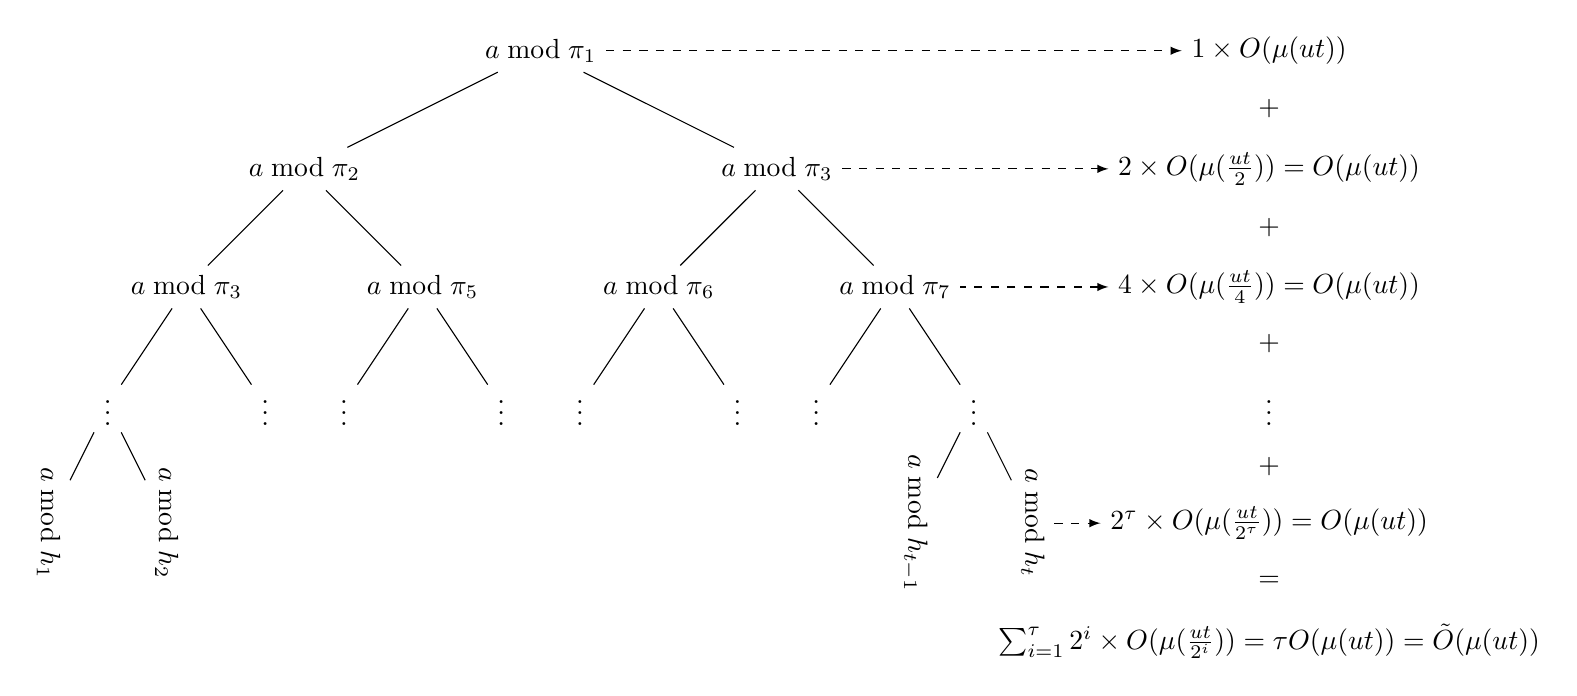
\begin{tikzpicture}[level/.style={sibling distance=60mm/#1}]
\node (z){$\displaystyle a \bmod \pi_1$}
  child {node (a) {$\displaystyle a \bmod \pi_2$}
    child {node (b) {$\displaystyle a \bmod \pi_3$}
      child {node {$\vdots$}
        child {node (d) {\begin{turn}{270}{$\displaystyle a \bmod h_{1}$}\end{turn}}}
        child {node (e) {\begin{turn}{270}{$\displaystyle a \bmod h_{2}$}\end{turn}}}
      }
      child {node {$\vdots$}}
    }
    child {node (g) {$\displaystyle a \bmod \pi_5$}
      child {node {$\vdots$}}
      child {node {$\vdots$}}
    }
  }
  child {node (j) {$\displaystyle a \bmod \pi_3$}
    child {node (k) {$\displaystyle a \bmod \pi_6$}
      child {node {$\vdots$}}
      child {node {$\vdots$}}
    }
    child {node (l) {$\displaystyle a \bmod \pi_7$}
      child {node {$\vdots$}}
      child {node (c){$\vdots$}
        child {node (o) {\begin{turn}{270}{$\displaystyle a \bmod h_{t-1}$}\end{turn}}}
        child {node (p) {\begin{turn}{270}{$\displaystyle a \bmod h_{t}$}\end{turn}}
%
%
          child [grow=right] {node (qe) {} edge from parent[draw=none]
            child [grow=right] {node (q) {$2^{\tau} \times O(\mu(\frac{ut}{2^{\tau}}))= O(\mu(u t))$} edge from parent[draw=none]
            child [grow=up] {node (r) {$\vdots$} edge from parent[draw=none]
            child [grow=up] {node (s) {$4 \times O(\mu(\frac{u t}4)) = O(\mu(u t))$} edge from parent[draw=none]
            child [grow=up] {node (t) {$2 \times O(\mu(\frac{u t}2)) = O(\mu(u t))$} edge from parent[draw=none]
            child [grow=up] {node (u) {$1 \times O(\mu(u t))$} edge from parent[draw=none]}
          }}}
          child [grow=down] {node (v) {$\sum_{i=1}^\tau 2^{i} \times O(\mu(\frac{ut}{2^i})) = \tau O(\mu(u t)) = \Oapp(\mu(u t))$}edge from parent[draw=none]}
            }
          }
        }
    }
  }
};
\path (q) -- (r) node [midway] {+};
\path (s) -- (r) node [midway] {+};
\path (s) -- (t) node [midway] {+};
\draw[<-,>=latex,dashed] (s) to (l);
\path (t) -- (u) node [midway] {+};
\draw[->,>=latex,dashed] (z) to (u);
\draw[->,>=latex,dashed] (j) to (t);
\draw[->,>=latex,dashed] (p) to (q);
\path (q) -- (v) node [midway] {$\displaystyle =$};
\end{tikzpicture}
\end{turn}}
\caption{Modular reduction from product tree (assuming $j=1$ for simplicity.}
\label{fig:div-prod-tree}
\end{figure}



% je ne comprends pas non plus (cf supra)
%\section{Implementation Details and Benchmarks}
%
%Tables~\ref{tab:benchdirec}, \ref{tab:rsyncopt} and~\ref{tab:results}.

\begin{table}
\begin{center}
\begin{tabular}{ll}\toprule
~~{\bf Directory}              ~~&~~{\bf Description}\\\midrule
~~{\tt synthetic}              ~~&~~A directory containing 1000 very small files containing~~\\
~~                             ~~&~~the numbers $1,2,\ldots,1000$. \\
~~{\tt synthetic\_shuffled}    ~~&~~{\tt synthetic} with:\\
                             ~~& ~~~~~10 deleted files\\
                             ~~& ~~~~~10 renamed files \\
                             ~~& ~~~~~10 modified files \\
~~{\tt source}                 ~~& ~~A snapshot of \btrsync's own source tree \\
~~{\tt source\_moved}          ~~& ~~{\tt source} with one big folder (a few megabits) renamed.~~\\
~~{\tt firefox-13.0}           ~~& ~~The source archive of Mozilla Firefox 13.0.\\
~~{\tt firefox-13.0.1}         ~~& ~~The source archive of Mozilla Firefox 13.0.1\\
~~{\tt empty}                  ~~& ~~An empty folder.\\\bottomrule
\end{tabular}\smallskip
  \caption{Test directories}
  \label{tab:benchdirec}
\end{center}
\end{table}

\begin{table}
  \begin{tabular}{p{\dimexpr 0.25\linewidth-2\tabcolsep} p{\dimexpr
    0.75\linewidth-2\tabcolsep}}
    \toprule
    $\blacktriangleright$ {\tt --delete} & Delete existing files on Oscar which
    do not exist on Neil like \btrsync does.\\
    $\blacktriangleright$ {\tt -I} & Ensure that \rsync does not cheat by
    looking at file modification times (which \btrsync does not do).\\
    $\blacktriangleright$ {\tt --chmod="a=rx,u+w"} & Attempt to disable the
    transfer of file permissions (which \btrsync does not transfer). Although
    these settings ensure that \rsync does not need to transfer permissions,
    verbose logging suggests that it does transfer them anyway, so \rsync must
    lose a few bytes per file as compared to \btrsync for this
    reason.\\
    $\blacktriangleright$ {\tt -v} & Count the number of sent and received
    bytes. For \btrsync we added a piece of code counting the amount of data
    transmitted during \btrsync's own negotiations.\\
    \bottomrule
  \end{tabular}\smallskip
  \caption{Options used when benchmarking \rsync}
  \label{tab:rsyncopt}
\end{table}

\begin{table}
  \setlength{\tabcolsep}{3pt}
  \begin{tabularx}{\textwidth}{ll X r r r r r r X r r }
    \toprule
    \multicolumn{2}{l}{\bf Entities and Datasets (see Table~\ref{tab:benchdirec})} &  &  \multicolumn{6}{c}{\bf Transmission (Bytes)} &  & \multicolumn{2}{r}{\bf Time (s)} \\
    \midrule {\bf Neil's $\mathfrak{F}'$}  & {\bf Oscar's $\mathfrak{F}$}
    & & $\mbox{{\tt TX}}_{\mbox{{\tiny {\tt rs}}}}$ & $\mbox{{\tt RX}}_{\mbox{{\tiny {\tt rs}}}}$  & $\mbox{{\tt TX}}_{\mbox{{\tiny {\tt bt}}}}$  & $\mbox{{\tt RX}}_{\mbox{{\tiny {\tt bt}}}}$  & $\delta_{\mbox{{\tiny {\tt rs}}}}-\delta_{\mbox{{\tiny {\tt bt}}}}$ &
    $\frac{\delta_{\mbox{{\tiny {\tt bt}}}}}{\delta_{\mbox{{\tiny {\tt rs}}}}}$ & & $\mbox{{\tt t}}_{\mbox{{\tiny {\tt rs}}}}$ & $\mbox{{\tt t}}_{\mbox{{\tiny {\tt bt}}}}$ \\\midrule
    %&&&&&&&&&&&\\[-1em]
    \texttt{source} & \texttt{empty} & 778311 & 1614 & 779517 & 10140 & 9732 & 1.0 & 0.1 & 0.4 \\
\texttt{empty} & \texttt{source} & 24 & 12 & 11927 & 5952 & 17843 & 496.6 & 0.1 & 0.4 \\
\texttt{empty} & \texttt{empty} & 24 & 12 & 19 & 30 & 13 & 1.4 & 0.0 & 0.3 \\
\texttt{synthetic} & \texttt{synthetic\_shuffled} & 54799 & 19012 & 7308 & 3417 & -63086 & 0.1 & 0.2 & 1.5 \\
\texttt{synthetic\_shuffled} & \texttt{synthetic} & 54407 & 18822 & 6822 & 3042 & -63365 & 0.1 & 0.2 & 0.8 \\
\texttt{synthetic} & \texttt{synthetic} & 54799 & 19012 & 327 & 30 & -73454 & 0.0 & 0.1 & 0.7 \\
\texttt{firefox-13.0.1} & \texttt{firefox-13.0} & 40998350 & 1187 & 39604079 & 3305 & -1392153 & 1.0 & 1.5 & 10.2 \\
\texttt{source\_moved} & \texttt{source} & 778176 & 1473 & 2757 & 1966 & -774926 & 0.0 & 0.1 & 0.6 \\

    \bottomrule
  \end{tabularx}\smallskip

  \caption{Experimental results. Synchronization is performed \textit{from} Neil \textit{to} Oscar. {\tt RX} and {\tt TX} denote the quantity of received and sent bytes, {\tt rs} and {\tt bt} denote {\tt rsync} and {\tt btrsync}, and $\delta_{\square}=\mbox{{\tt TX}}_{\square}+\mbox{{\tt RX}}_{\square}$. $\delta_{\mbox{{\tiny {\tt rs}}}}-\delta_{\mbox{{\tiny {\tt bt}}}}$ and ${\delta_{\mbox{{\tiny {\tt bt}}}}}/{\delta_{\mbox{{\tiny {\tt rs}}}}}$ express the absolute and the relative differences in transmission between \rsync and \btrsync. The last two columns show timing results on an Intel Core i3-2310M CPU clocked at 2.10 Ghz.}
  \label{tab:results}
\end{table}



\end{document}
